%! Licence = CC BY-NC-SA 4.0

%! Author = gianfluetsch
%! Date = 22. Jan 2022
%! Project = icth_summary

\section{Signale}
\subsubsection{Begriffe}
\textbf{Kehrlage}\\
Kehrlage bezeichnet entsprechend das tieffrequentere (untere) Seitenband.

\textbf{Regellage}\\
Die Regellage bezeichnet das hochfrequentere (obere) Seitenband einer amplitudenmodulierten Funkträgerwelle, deren jeweilige Schwingungsfrequenz sich aus der Summe der Träger- und momentanen Signalfrequenz ergibt.\\

\begin{center}
    \vspace{-8pt}
    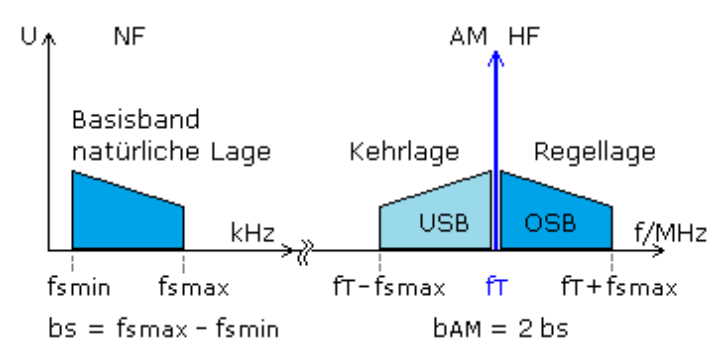
\includegraphics[width=.6\linewidth]{./03-signale/kehrlage_regellage}
    \vspace{-8pt}
\end{center}

\textbf{Präambel}\\
\begin{itemize}
    \item ist ein Signal, das in einem Rechnernetz übertragenen Nachrichten vorangestellt wird
    \item im Gegensatz zum Header eines Datenpakets gehört die Präambel nicht zu den Daten selbst, sondern dient der Abstimmung der Gesprächspartner im Netz
    \item bei serieller Übertragung folgt nach der Präambel bzw. an deren Ende häufig eine bestimmte Bitfolge, die den Beginn der eigentlichen Daten ankündigt und eine Synchronisation auf die Wortgrenze ermöglicht\\
\end{itemize}

\textbf{Wozu wird eine Präambel einem codierten Datenpaket vorangestellt?}\\
Die Präambel dient der Frequenz und Phasensynchronisation. So wird sichergestellt, dass die Abtastung immer zum richtigen Zeitpunkt erfolgt.\\

\textbf{Nachteil, wenn Länge der Präambel über Zeit definiert wird und Übertragungsrate bei gleicher (konstanter) Datenblockgrösse steigt?}\\
Die Präambel wird im Verhältnis zur Datenblockgrösse grösser, das heisst, der Overhead pro gesendeten Datenpaket steigt und es kann nicht die maximale Netto-Datenrate erreicht werden. Ein Beispiel für diesen Effekt ist im WLAN eindrücklich gegeben.\\

\subsubsection{A}
\textbf{Um wie viel dB muss ein Signal verstärkt werden, wenn der Ausgangspegel}
\begin{enumerate}
    \item doppelt so gross sein soll wie der Eingangspegel
    \item viermal so gross sein soll wie der Eingangspegel
\end{enumerate}

$v=10*log_{10}(\frac{U_{out}}{U_{in}}) \rightarrow v=Verstärkung, [v]=dB$\\
1)$v=10*log_{10}(\frac{1}{2})=3.0103dB$\\
2)$v=10*log_{10}(\frac{4}{1})=6.0206dB$\\

\textbf{Ein Eingangssignal wird durch eine Leitung um 6 dB gedämpft. Um das wie viel Fache ist der Ausgangspegel kleiner als der Eingangspegel?}\\
$v=-6dB$\\
$-6dB=10*log_{10}(\frac{U_{out}}{1}) \rightarrow U_{out}=0.251189 = 25\%$\\
Der Ausgangspegel entspricht etwa 1/4 des Eingangspegels.\\

\textbf{Schallwellen Ohr}\\
Seine Schallwellen haben zu ihrem rechten Ohr einen Weg zurückzulegen, der etwa l = 23 cm l¨anger ist als zu ihrem linken Ohr. Die dadurch bedingte Verzögerung
lässt sich für Sinustöne durch eine Phasenverschiebung darstellen\\
\begin{itemize}
    \item Signal am linken Ohr: $x_l(t)=X_lsin(\omega t)$
    \item Signal am rechten Ohr: $x_r(t)=x_tsin(\omega t+\varphi )$\\
\end{itemize}

Wie gross ist der Laufzeitunterschied $\tau$ der Schallwellen zwischen dem linken und dem rechten Ohr? (Schallgeschwindigkeit c = 340 m/s)\\
$\tau =\frac{l}{c}=\frac{0.23}{340}s=0.676ms$\\

Wie gross ist die Phasenverschiebung jeweils für Sinustöne der Frequenzen 100 Hz, 200 Hz, 1 kHz?\\
$\varphi =2\pi \frac{s}{\lambda }=s\pi \frac{s*f}{c}=2\pi \tau f$\\
$\varphi_1=2\pi * 0.000676*100=0.135\pi$\\
$\varphi_2=2\pi * 0.000676*200=0.270\pi$\\
$\varphi_3=2\pi * 0.000676*1000=1.35\pi$\\

Bei welcher Frequenz entspricht die Phasenverschiebung genau einer Periode der Schwingung?\\
\textit{Die Phasenverschiebung muss genau $2\pi$ betragen.}\\
$\varphi = 2\pi \tau f = 2\pi$\\
$f=\frac{1}{\tau}=1.48kHz$\\

Erklären Sie anhand der frequenzabhängigen Phasenverschiebung, warum ein Subwoofer an einem beliebigen Ort des Raumes stehen darf und der Stereoeffekt dadurch nicht beeinflusst wird?\\
\textit{Das Gehirn misst zur Lokalisierung der Richtung, aus der ein Ton kommt, den Phasenunterschied zwischen linkem und rechtem Ohr (Triangulationsmessung). Bei tiefen Frequenzen ist der Phasenunterschied so gering, dass das Ohr ihn nicht mehr aufl¨osen kann. Daher kann der Subwoofer ihrer Stereoanlage irgendwo im Raum stehen, ohne ihr H¨orvergn¨ugen zu beeinträchtigen.}

\subsubsection{B}
Sie planen einen Subwoofer zu bauen und wissen, dass die minimale Phasenverschiebung zwischen dem linken und rechten Ohr, die ein Mensch zur Lokalisierung der Schallquelle noch auswerten kann bei 0.2 rad liegt.
Bestimmen sie die obere Grenzfrequenz, die der Subwoofer maximal abgeben darf.\\

Gehen sie dabei von den folgenden Annahmen aus. Der Abstand von einem Ohr zum anderen ist  im Mittel mit 21 cm gegeben. Die Schallgeschwindigkeit wird mit 330 m/s angenommen.\\

\textbf{Stellen sie die maximale Phasenverschiebung des Audiosignals von einem zum anderen Ohr als Funktion der Frequenz dar.\\}
$\phi(f)=2\pi f s/v = f = \frac{\phi}{2\pi}*\frac{s}{v}$\\
$f=\frac{0.2*330 m/s}{2\pi*0.21m} = 50 Hz$\\

Fourier:  Gegeben ist ein Generator der folgendes Dreieckssignal mit der Frequenz von 3 kHz generiert:
\begin{center}
    \vspace{-8pt}
    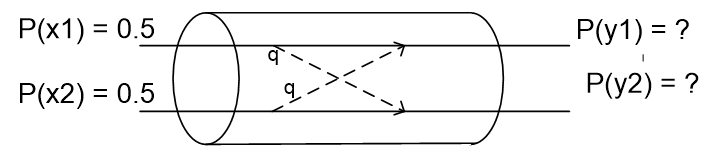
\includegraphics[width=.6\linewidth]{./03-signale/fs2015}
    \vspace{-8pt}
\end{center}

\textbf{Sie wollen ein harmonisches Signal mit der Frequenz von 9 kHz erzeugen. Entwickeln Sie eine Prinzipschaltung unter Angabe aller signifikanten Werte, die dies realisiert.}\\
$y(t)=\frac{8\hat{y}}{\pi^2}(\frac{1}{1^2}*sin(\Omega_0 t)-\frac{1}{3^2}*sin(3\Omega_0 t)+\frac{1}{5^2}*sin(5\Omega_0 t)-...)$\\
\textit{Die Frequenz von 9 kHz entspricht der zweiten harmonischen $\rightarrow$ durch einen Bandpass mit der unteren Grezfrequenz von z.B. 8 khz und einer oberen Grenzfrequenz von z. Bsp 10 kHz }\\

\textbf{Wie gross ist die Amplitude dieser harmonischen Schwingung?}\\
$a=\frac{8*10V}{9*\pi^2}=0.9V$\\

\textbf{Um wie viel db ist dann das Ausgangssignal gegenüber dem Eingangssignal gedämpft?}\\
$a=10log\frac{0.9V}{10V}=-10.46db$\\

\textbf{Wie hoch ist dann der Pegel in V beim Empfänger, wenn die nachgeschaltete Übertra-gungsstrecke eine Dämpfung von 3 db aufweist?}\\
$-13.46db = 10log\frac{x}{10}$\\
$10^{-1.346}*10V = 0.045V$

\subsubsection{C}
Zur Verschleierung von Sprachsignalen wird das System in Bild unten, auch Scrambler genannt, eingesetzt. Es transformiert das Signalspektrum in die Kehrlage und wurde beispielweise im Mobilfunknetz C eingesetzt.\\
\begin{center}
    \vspace{-8pt}
    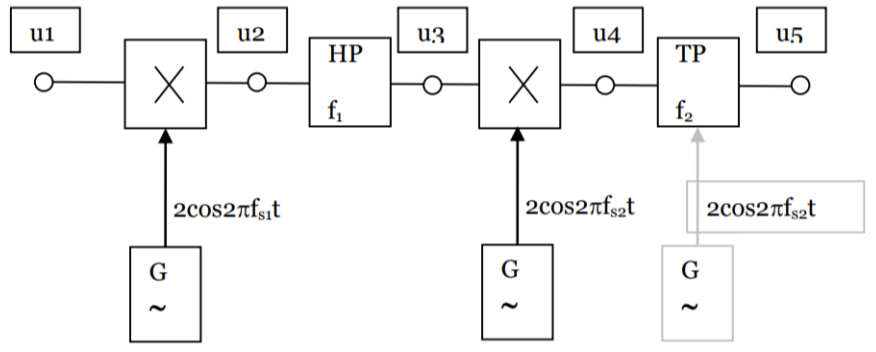
\includegraphics[width=.6\linewidth]{./03-signale/hs2009_6}
    \vspace{-8pt}
\end{center}

\textbf{Was versteht man unter Kehrlage eines Signals?}\\
Das höherfrequente Nachchtensignal liegt in beiden Seitenbändern näher bei der Trägerfrequenz als das niedfrequente Nachrichtensignal.\\

Analysieren Sie das System, indem Sie die Spektren der Signale u1 bis u5 skizzieren. Es ist g die Grenzfrequenz des Eingangssignals u1.\\
Geben Sie ferner die Frequenzen f1, f2 sowie fs1 und fs2 zueinander so an, dass der Scrambler seine Aufgabe erfüllen kann.
\begin{center}
    \vspace{-8pt}
    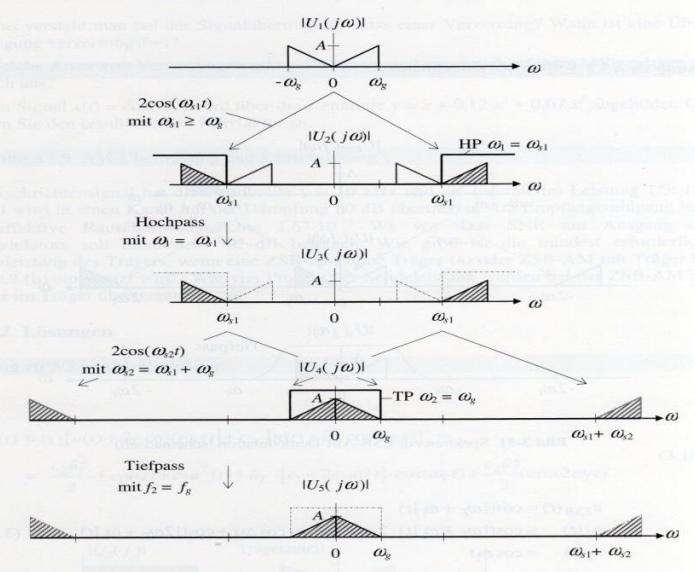
\includegraphics[width=.6\linewidth]{./03-signale/hs2009_7}
    \vspace{-8pt}
\end{center}

Gegeben ist das folgende Spektrum eines modulierten Sprachsignals.
\begin{center}
    \vspace{-8pt}
    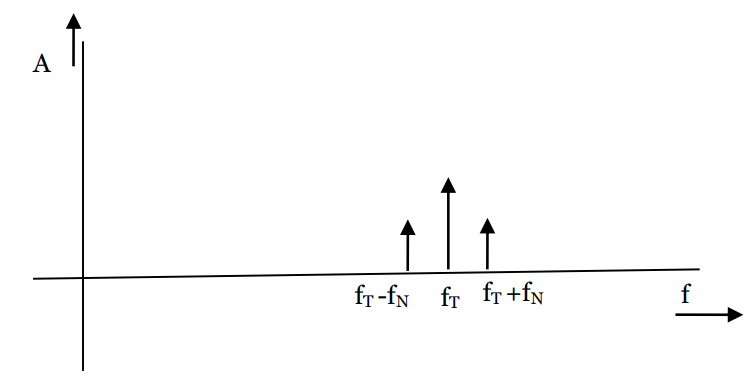
\includegraphics[width=.6\linewidth]{./03-signale/hs2009_8}
    \vspace{-8pt}
\end{center}

\textbf{Befindet sich das Sprachsignal fN in der Kehr- oder Regellage? (Anm. die Frequenz fN ist die obere Grenzfrequenz des Sprachsignals)}\\
Das Signal befindet sich nicht in der Kehrlage.\\

Konstruieren Sie eine Demodulatoschaltung und zeigen sie rechnerisch, dass das Sprachsignal fN im Basisband vorliegt.\\
\begin{center}
    \vspace{-8pt}
    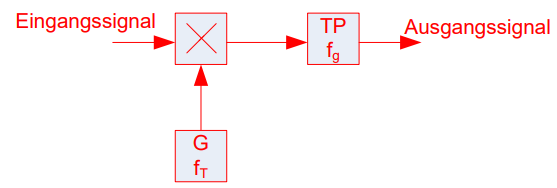
\includegraphics[width=.6\linewidth]{./03-signale/hs2009_9}
    \vspace{-8pt}
\end{center}

\begin{center}
    \vspace{-8pt}
    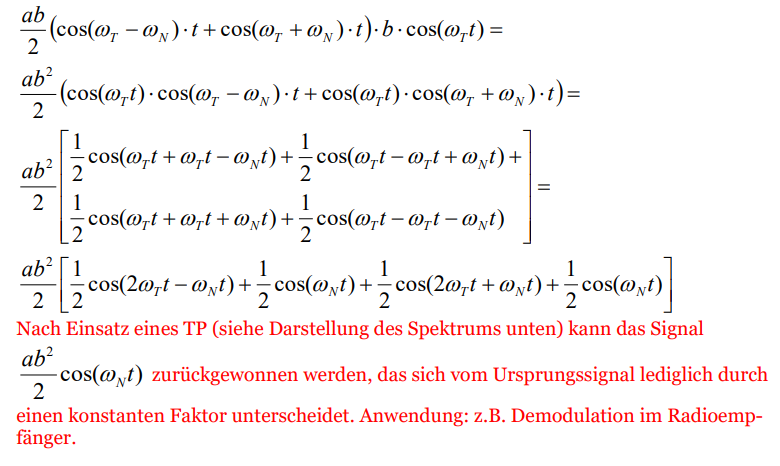
\includegraphics[width=.8\linewidth]{./03-signale/hs2009_10}
    \vspace{-8pt}
\end{center}

\columnbreak

\subsubsection{D}
Gegeben ist das folgende Blockschaltbild:
\begin{center}
    \vspace{-8pt}
    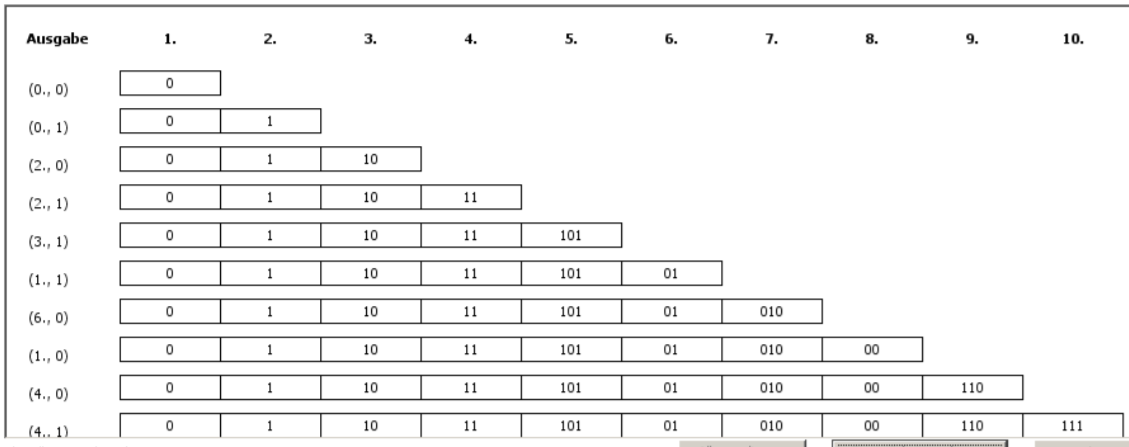
\includegraphics[width=.8\linewidth]{./03-signale/fs2009}
    \vspace{-8pt}
\end{center}

\textbf{Zeichnen Sie das Frequenzspektrum, das Sie an dem Punkt1, dem Punkt 2 und dem Punkt 3 beobachten können.}\\
Die Fourierzerlegung folgt für\\
$f(x)=a(sin(x)+\frac{sin(2x)}{2}+\frac{sin(3x)}{3}+...)$\\

Das positive Sägezahnsignal zu:\\
$f(x)=a(\frac{1}{1^2}*sin(x)-\frac{sin(3x)}{3^2}+\frac{sin(5x)}{5^2}-....)$\\

Und das Dreieckssignal zu:
\begin{center}
    \vspace{-8pt}
    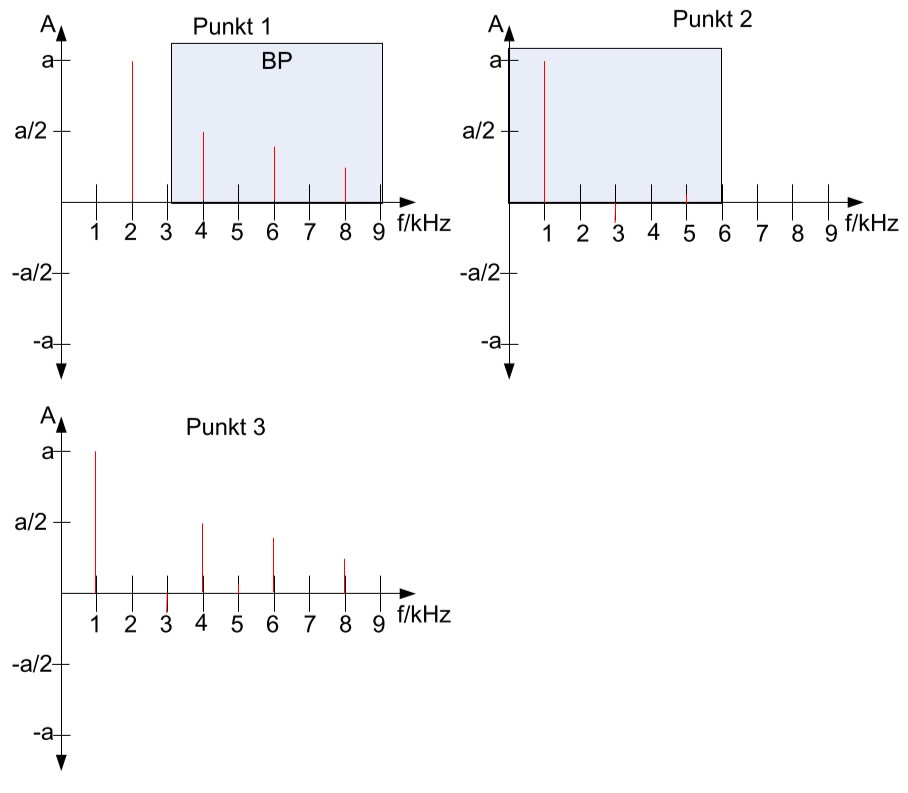
\includegraphics[width=.8\linewidth]{./03-signale/fs2009_2}
    \vspace{-8pt}
\end{center}

\subsubsection{E}
\textbf{Entwickeln sie eine Schaltung, die ihre natürliche Sprache in einen höheren Frequenzbereich transponiert (”Heliumeffekt”).}\\
Die Idee ist einfach umzusetzen, wenn man das Ganze im Frequenzbereich betrachtet. Nehmen wir an, dass das Sprachsignal auf z.B 16kHz beschränkt wird, da wir darüber hinaus nichts mehr hören. 
Dann ergibt sich das in unten dargestellte Frequenzspektrum der Sprache. Um den gewünschten ''Heliumeffekt'' zu erzielen, muss das Spektrum geringfügig verschoben werden. 
Dies wird durch die Multiplikation mit einem Trägersignal erreicht. Da durch die Multiplikation ein oberes und ein unteres Seitenband entstehen ist eine einfache Verschiebung um nur 100
bis 200 Hz nicht möglich, ohne Störungen in den hörbaren Bereich zu erhalten.\\
\begin{center}
    \vspace{-8pt}
    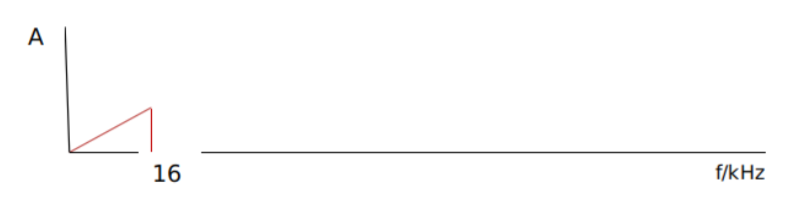
\includegraphics[width=.8\linewidth]{./03-signale/w13}
    \vspace{-8pt}
\end{center}

Daher wird das Signal erst einmal in einen höheren Bereich transponiert, d.h. mit einer Frequenz von z.B. 40 kHz multipliziert. 
Das resultierende Spektrum ergibt sich dann zu:
\begin{center}
    \vspace{-8pt}
    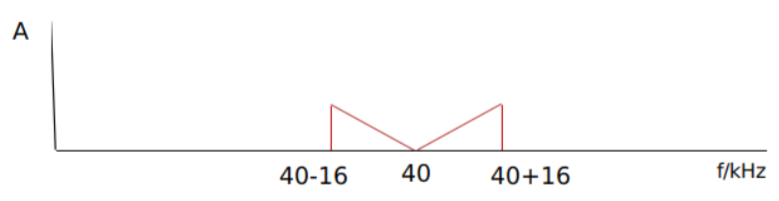
\includegraphics[width=.8\linewidth]{./03-signale/w13_2}
    \vspace{-8pt}
\end{center}

Würde es nun wieder mit 40 kHz multipliziert, würde sich wiederum das ursprüngliche Signal ergeben (siehe frühere Übung). 
Wir möchten jedoch eine Verschiebung in den höheren Bereich erreichen und daher mit einer etwas geringeren Frequenz, z.B. 39.9 kHz multiplizieren. 
Wenn wir das machen, werden die beiden Seitenb¨ander aber unterschiedlich verschoben (± die 100 Hz). Um das zu verhindern, muss erst ein Seitenband wegeschnitten werden. 
Mit diesen ergibt sich die folgende Lösung:
\begin{center}
    \vspace{-8pt}
    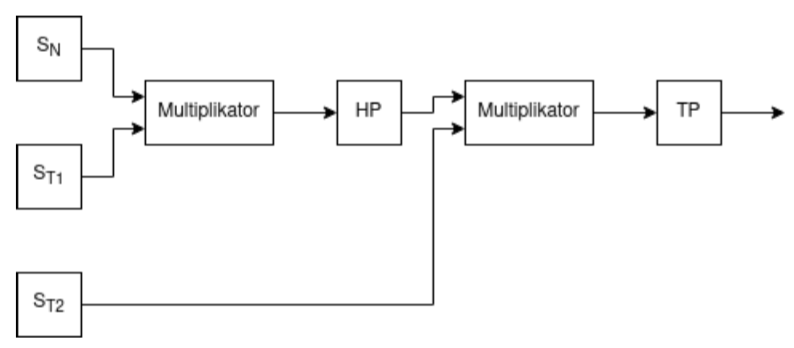
\includegraphics[width=.8\linewidth]{./03-signale/w13_3}
    \vspace{-8pt}
\end{center}

Mathematisch:\\
$S=S_{T2}*(S_{T1}*S_N)=cos(\omega_{T2}t)(cos((\omega_{T1}-\omega_N)t)+cos((\omega_{T1}+\omega_N)t))$\\
$=cos((\omega_{T2}+\omega_{T1}-\omega_N)t)+cos((\omega_{T2}-\omega_{T1}+\omega_N)t)$\\
$+cos((\omega_{T2}+\omega_{T1}+\omega_N)t)+cos((\omega_{T2}-\omega_{T1}-\omega_N)t)$\\

Mit einem Tiefpass nach der Demodulation bleibt mit $\Delta \omega = \omega_{T1}-\omega_{T2}$:\\
$S=cos((\omega_{T2}-\omega_{T1}+\omega_N)t)+cos((\omega_{T2}-\omega_{T1}-\omega_N)t)$\\
$=cos((-\Delta \omega + \omega_N)t)+cos((-\Delta \omega -\omega_N)t)$\\
$=cos((\omega_N-\Delta \omega)t)+cos((\omega_N+\Delta \omega)t)$\\

Für den gewünschten Effekt müssen wir also z.B. den ersten Term verschwinden lassen. Da dieser durch das untere Seitenband nach der Modulation entsteht,
setzen wir an dieser Stellen entsprechend einen Hochpass ein.\\

\textbf{Entwickeln sie eine Schaltung, auf der drei Telefongespräche (4kHz) über eine Leitung gemultiplext werden können.}\\
Die Gespräche können nur dann fehlerfrei übertragen werden, wenn sie sich nicht gegenseitig stören. Da die Gespräche gleichzeitig zu übertragen sind, ist das im Zeitbereich nicht möglich. 
Hat das Übertragungsmedium jedoch eine genügend hohe Bandbreite, so kann ein Frequenzmultiplex durchgeführt werden. Dazu sind die Gespräche 2 und 3 in ein höheres Band zu transponieren. Gespräch 1 kann im Basisband bleiben. 
Das kann einfach durch die Multiplikation mit einem Trägersignal erreicht werden. Aus der Abbildung unten lassen sich unmittelbar die erforderlichen Modulationsfrequenzen ableiten, wenn man zugrunde legt, dass
sich die Frequenzspektren nicht überlappen dürfen.
\begin{center}
    \vspace{-8pt}
    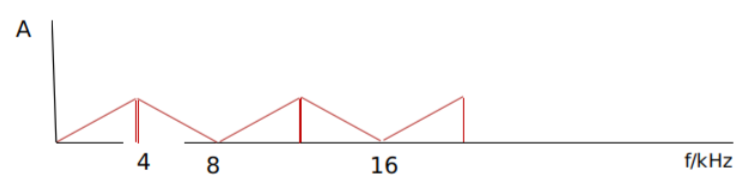
\includegraphics[width=.8\linewidth]{./03-signale/w13_4}
    \vspace{-8pt}
\end{center}

Beide modulierten Signale besitzen eine Bandbreite von $B=2*4kHz=8kHz$, die Trägerfrequenz sind dementsprechend $f_{T1}=8kHz$ und $f_{T2}=16kHz$.
\begin{center}
    \vspace{-8pt}
    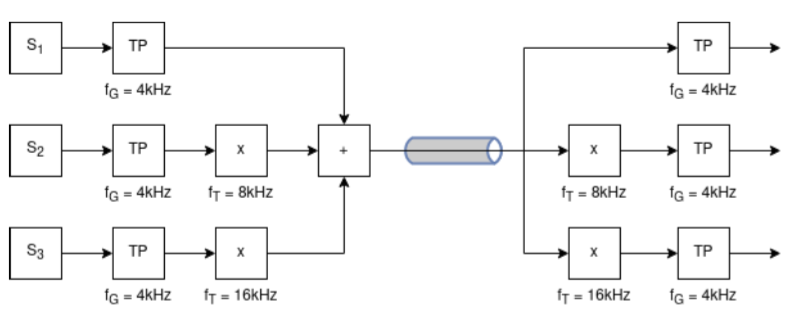
\includegraphics[width=.8\linewidth]{./03-signale/w13_5}
    \vspace{-8pt}
\end{center}
